\documentclass[10pt]{beamer}

% mac版,texShop 中Typeset选择 XeLaTex 

%%%%%%%%%%%%%%%%%%%%%%%%%%%%%%%%%%%%%
\usepackage[slantfont,boldfont]{xeCJK}
%\input{xecjkfonts},CJKtextspaces
\setCJKmainfont{STKaiti}   % STFangsong 设置缺省中文字体
\setCJKmonofont{SimSun}   % 设置等宽字体
\setmainfont{Times} % 英文衬线字体
\setmonofont{Times} % 英文等宽字体
\setsansfont{Times} % 英文无衬线字体
%%%%%%%%%%%%%%%%%%%%%%%%%%%%%%%%%%%%%%

\mode<presentation> {
  %\usetheme{Madrid}
  %\usetheme{Singapore}
  \usetheme{Warsaw}
  \setbeamercovered{transparent}
 % \usefonttheme[onlymath]{serif}  
 \usefonttheme{professionalfonts}%{structurebold}
 % \usefonttheme[onlymath]{structurebold}
  \usecolortheme{rose}
}

\usepackage[english]{babel}
%\usepackage[latin1]{inputenc}

%\usepackage{times}
%\usepackage[T1]{fontenc}


%\usepackage{epsfig}
\usepackage{graphics}
\usepackage{color}
\usepackage{amsmath,amssymb,mathrsfs}
\usepackage{amsfonts,stmaryrd}
%\usepackage{thmmarks}
%\usepackage{}



\newcommand\frakfamily{\usefont{U}{yfrak}{m}{n}}
\DeclareTextFontCommand{\textfrak}{\frakfamily}
\def\diag{\mathrm{diag}}


\title[数值计算方法]{数值计算方法}
\subtitle{-离散傅立叶变换和三角插值}


\subject{Talks}

% If you have a file called "university-logo-filename.xxx", where xxx
% is a graphic format that can be processed by latex or pdflatex,
% resp., then you can add a logo as follows:

% \pgfdeclareimage[height=0.5cm]{university-logo}{university-logo-filename}
% \logo{\pgfuseimage{university-logo}}

%\pgfdeclareimage[height=0.5cm]{university-logo}{ncsu_logo}
%\logo{\pgfuseimage{university-logo}}

% Delete this, if you do not want the table of contents to pop up at
% the beginning of each subsection:
%\AtBeginSubsection[] {
%  \begin{frame}<beamer>
%    \frametitle{Outline}
%    \tableofcontents[currentsection,currentsubsection]
%  \end{frame}
%}

% If you wish to uncover everything in a step-wise fashion, uncomment
% the following command:

% \beamerdefaultoverlayspecification{<+->}


\setbeamertemplate{theorems}[numbered]
\setbeamertemplate{caption}[numbered]


\newtheorem{proposition}[theorem]{Proposition}

%%%%%%%%%%%%%%%%%%%%%%%%%%%
% REMARK-STYLE-ENVIRONMENTS %
%%%%%%%%%%%%%%%%%%%%%%%%%%%
\newcounter{remark}
% \numberwithin{theorem}{section}
\def\openrem#1#2{\refstepcounter{remark}\bigskip

{\noindent\bf#1~\theremark\if#2!{. }\else{ (#2).}\fi}
\it}
\def\thmskip{}
\newenvironment{remark}[1][!]{\openrem{Remark}{#1}}{\thmskip}

%%%%%%%%%%%%%%%%%%%%%%%%%%%%
%% AlGORITHM-STYLE-ENVIRONMENTS %
%%%%%%%%%%%%%%%%%%%%%%%%%%%%
\newcounter{algorithm}
% \numberwithin{theorem}{section}
\def\openalg#1#2{\refstepcounter{algorithm}\bigskip

{\noindent\bf#1~\thealgorithm\if#2!{. }\else{ (#2).}\fi}
\it}
\def\thmskip{}
\newenvironment{algorithm}[1][!]{\openrem{Algorithm}{#1}}{\thmskip}
%
%
%%%%%%%%%%%%%%%%%%%%%%%%%%%%
%% Result-STYLE-ENVIRONMENTS %
%%%%%%%%%%%%%%%%%%%%%%%%%%%%
%\newcounter{result}
%\def\openrem#1#2{\refstepcounter{result}\bigskip
%{\noindent \it \bfseries#1~\theremark\if#2!{. }\else{ (#2). }\fi}}
%\newenvironment{result}[1][!]{\openrem{Result}{#1}}{\qed}




%%%%%%%%%%%%%%%%%%%%%%%%%%%
%Redefine the Symbols%
%%%%%%%%%%%%%%%%%%%%%%%%%%%

\def\mathbi#1{\textbf{\em #1}}

% integrals
\def\dx{\,{\rm d}x}
\def\dxb{\,{\rm d}\boldsymbol{x}}
\def\dy{\,{\rm d}y}
\def\dt{\,{\rm d}t}
\def\ds{\,{\rm d}s}
\def\du{\,{\rm d}u}

\def\dr{\,{\rm d}r}
\def\dtheta{\,{\rm d}\theta}

\def\dd{{\rm d}}

\def\intOm{\int_{\Omega}}
\def\intbOm{\int_{\partial \Omega}}

% differences
\def\Dx{\Delta x}
\def\Dt{\Delta t}
\def\D{\Delta}


% operators
\def\Ls{\mathscr{L}}

% matirices
\def\Js{\mathscr{J}}


%fields%
\def\R{\mathbb{R}}
\def\N{\mathbb{N}}
\def\Z{\mathbb{Z}}

%Spaces%
\def\H{\mathbb{H}}
\def\L{\mathbb{L}}
\def\P{\mathbb{P}}


\def\U{\mathbb{U}}
\def\V{\mathbb{V}}
\def\W{\mathbb{W}}
\def\X{\mathbb{X}}
\def\Y{\mathbb{Y}}

\def\Cinfty{C^\infty}




%vectors%
\def\ab{\boldsymbol{a}}
\def\bb{\boldsymbol{b}}
\def\cb{\boldsymbol{c}}
\def\db{\boldsymbol{d}}
\def\eb{\boldsymbol{e}}
\def\fb{\boldsymbol{f}}
\def\gb{\boldsymbol{g}}
\def\hb{\boldsymbol{h}}
\def\nb{\boldsymbol{n}}
\def\rb{\boldsymbol{r}}
\def\sb{\boldsymbol{s}}


\def\ub{\boldsymbol{u}}
\def\vb{\boldsymbol{v}}
\def\wb{\boldsymbol{w}}
\def\xb{\boldsymbol{x}}
\def\yb{\boldsymbol{y}}
\def\zb{\boldsymbol{z}}

\def\Bb{\boldsymbol{B}}
\def\Cb{\boldsymbol{C}}
\def\Eb{\boldsymbol{E}}
\def\Fb{\boldsymbol{F}}
\def\Ib{\boldsymbol{I}}
\def\Kb{\boldsymbol{K}}
\def\Ob{\boldsymbol{O}}
\def\Qb{\boldsymbol{Q}}
\def\Rb{\boldsymbol{R}}
\def\Sb{\boldsymbol{S}}
\def\Ub{\boldsymbol{U}}
\def\Vb{\boldsymbol{V}}
\def\Wb{\boldsymbol{W}}
\def\Xb{\boldsymbol{X}}
\def\Yb{\boldsymbol{Y}}
\def\Zb{\boldsymbol{Z}}

%domains%
\def\Om{\Omega}
\def\bd{\partial}
\def\bOm{\bar{\Omega}}

%bold symbols%
\def\alphab{\boldsymbol{\alpha}}
\def\phib{\boldsymbol{\varphi}}

%energy%
\def\Jc{\mathcal{J}}
\def\Oc{\mathcal{O}}

%Greeks%
\def\vphi{\varphi}

%Special Functions%
\def\supp{\rm{supp}}
\def\sym{\rm{sym}}

\def\gradu{\nabla u}
\def\gradv{\nabla v}

%Mesh%
\def\Ts{\mathcal{T}}

\def\mach{\rm{mach}}


\begin{document}

\setbeamertemplate{itemize item}[triangle]

\begin{frame}
\titlepage
\end{frame}


\begin{frame}
  \frametitle{本节概要}
  \tableofcontents%[pausesections]
  % You might wish to add the option [pausesections]
%  \begin{itemize}
%  \item 显示Euler法及其误差分析
%  \item Taylor展开法
%  \item 
%  \end{itemize}
\end{frame}

\section{离散傅立叶变换}

\begin{frame}
\frametitle{傅立叶变换}
\begin{definition}[傅立叶变换]
如果函数$f$是连续可微的,且$\int_{-\infty}^{+\infty} |f(t)| \dt < +\infty$,则函数的离散傅立叶变换为
\begin{equation}
\hat{f}(\lambda) = \frac{1}{\sqrt{2\pi}}\int_{-\infty}^{+\infty} f(t) e^{-i \lambda t} \dt.
\end{equation}
\end{definition}
现在假设当$x<a, x>b$时,$f(x) = 0$,且$f(a) = f(b)$,则
\begin{equation}
\hat{f}(\lambda)= \frac{1}{\sqrt{2\pi}}\int_{-\infty}^{+\infty} f(t) e^{-i \lambda t} \dt =  \frac{1}{\sqrt{2\pi}}\int_{a}^{b} f(t) e^{-i \lambda t} \dt.
\end{equation}
\end{frame}


\begin{frame}
\frametitle{傅立叶变换}
现在令$\theta = 2\pi\frac{t-a}{b-a}$,则
\begin{equation}
\hat{f}(\lambda)= \frac{b-a}{(2\pi)^{\frac{3}{2}}} e^{-i \lambda a} \int_0^{2\pi} f(a + \frac{(b-a) \theta}{2\pi}) e^{\frac{(b-a) \lambda}{2\pi}\theta} \dd \theta.
\end{equation}
令
\begin{equation}
g(\theta) : =  f(a + \frac{(b-a) \theta}{2\pi}) \text{ 以及 } \lambda_k = \frac{2\pi}{b-a} k,
\end{equation}
则$\hat{f}(\lambda_k)$就变成了
\begin{equation}
\hat{f}(\lambda_k) = \frac{b-a}{\sqrt{2\pi}} e^{-i \lambda_k a} \big\{ \frac{1}{\sqrt{2\pi}} \int_0^{2\pi} g(\theta) e^{-i k \theta} \dd \theta \big\}.
\end{equation}
\end{frame}


\begin{frame}
\frametitle{离散傅立叶变换的导出}
对区间$[0, 2\pi]$进行$n$等分,对积分
\begin{equation}
\frac{1}{2\pi} \int_0^{2\pi} g(\theta) e^{-i k \theta} \dd \theta,
\end{equation}
使用复合梯形公式并利用$g(0) = g(2\pi)$(即$f(a) = f(b)$)得到
\begin{align}
&\frac{1}{2\pi} \int_0^{2\pi} g(\theta) e^{-i k \theta} \dd \theta \nonumber\\
= &\frac{1}{2\pi} \frac{2\pi}{n} \Big[ \frac{1}{2}(g(0)e^{-i k \frac{2\pi}{n}0} + g(\frac{2\pi}{n})e^{-i k \frac{2\pi}{n}1}) \nonumber \\
& +  \frac{1}{2}(g(\frac{2\pi}{n})e^{-i k \frac{2\pi}{n}1} + g(\frac{2\pi}{n}2)e^{-i k \frac{2\pi}{n}2}) \nonumber \\
& + \ldots \nonumber \\
&+ \frac{1}{2}(g(\frac{2\pi}{n}(n-1))e^{-i k \frac{2\pi}{n}(n-1)} + g(\frac{2\pi}{n}n)e^{-i k \frac{2\pi}{n}(n)}) \Big] \nonumber \\
=& \frac{1}{n} \sum_{j = 0}^{n-1} g(\frac{2\pi}{n}j) e^{-i  \frac{2\pi}{n}jk}.
\end{align}
\end{frame}


\begin{frame}
\frametitle{离散傅立叶变换}
更一般的,我们设$x = [x_0, \ldots, x_{n-1}]^T$为$n-$维向量,令$\omega = e^{-i \frac{2\pi}{n}}$。
\begin{definition}[离散傅立叶变换]
对于$n-$维向量$x = [x_0, \ldots, x_{n-1}]^T$,其离散傅立叶变换也是一个$n-$维向量$y = [y_0, \ldots, y_{n-1}]^T$,满足
\begin{equation}
\label{eq: DFT original}
y_k = \frac{1}{\sqrt{n}} \sum_{j = 0}^{n-1} x_j \omega^{jk},
\end{equation}
其中$\omega = e^{-i \frac{2\pi}{n}}$。
\end{definition}
\end{frame}


\begin{frame}
\frametitle{离散傅立叶变换的矩阵形式}
将上面的定义可以写为矩阵形式
\begin{align*}
\left[ \begin{array}{c}
     y_0 \\ y_1 \\y_2 \\ \vdots \\ y_{n-1}  \end{array} \right]
=& \frac{1}{\sqrt{n}} \left[ \begin{array}{ccccc}
     \omega^0    &  \omega^0 &  \omega^0 & \cdots &  \omega^0  \\
     \omega^0    &  \omega^1 &  \omega^2 & \cdots &  \omega^{n-1}  \\
     \omega^0    &  \omega^2 &  \omega^4 & \cdots &  \omega^{2(n-1)}  \\
     \omega^0    &  \omega^3 &  \omega^6 & \cdots &  \omega^{3(n-1)}  \\
     \vdots    &  \vdots & \vdots &\quad &  \vdots  \\
     \omega^0    &  \omega^{n-1} &  \omega^{2(n-1)} & \cdots &  \omega^{(n-1)^2}  \\                   
            \end{array} \right] 
\left[ \begin{array}{c}
     x_0 \\ x_1 \\ x_2 \\ \vdots \\ x_{n-1}  \end{array} \right].
\end{align*}
我们称右端第一个矩阵为傅立叶矩阵
\begin{align}
F_n = & \frac{1}{\sqrt{n}} \left[ \begin{array}{ccccc}
     \omega^0    &  \omega^0 &  \omega^0 & \cdots &  \omega^0  \\
     \omega^0    &  \omega^1 &  \omega^2 & \cdots &  \omega^{n-1}  \\
     \omega^0    &  \omega^2 &  \omega^4 & \cdots &  \omega^{2(n-1)}  \\
     \omega^0    &  \omega^3 &  \omega^6 & \cdots &  \omega^{3(n-1)}  \\
     \vdots    &  \vdots & \vdots &\quad &  \vdots  \\
     \omega^0    &  \omega^{n-1} &  \omega^{2(n-1)} & \cdots &  \omega^{(n-1)^2}  \\                   
            \end{array} \right] .
\end{align}
\end{frame}


\begin{frame}
\frametitle{离散傅立叶逆变换}
对于通过公式\eqref{eq: DFT original}得到的向量$y = [y_0, \ldots, y_{n-1}]$,如果我们在其左侧乘以$F_n$矩阵的逆$F_n^{-1}$,得到的向量就是$x$本身,即$x = F_n^{-1} y$。这个过程称为离散傅立叶逆变换。事实上我们可以证明
\begin{align}
F^{-1}_n = & \frac{1}{\sqrt{n}} \left[ \begin{array}{ccccc}
     \omega^0    &  \omega^0 &  \omega^0 & \cdots &  \omega^0  \\
     \omega^0    &  \omega^{-1} &  \omega^{-2} & \cdots &  \omega^{-(n-1)}  \\
     \omega^0    &  \omega^{-2} &  \omega^{-4} & \cdots &  \omega^{-2(n-1)}  \\
     \omega^0    &  \omega^{-3} &  \omega^{-6} & \cdots &  \omega^{-3(n-1)}  \\
     \vdots    &  \vdots & \vdots &\quad &  \vdots  \\
     \omega^0    &  \omega^{-(n-1)} &  \omega^{-2(n-1)} & \cdots &  \omega^{-(n-1)^2}  \\                   
            \end{array} \right] ,
\end{align}
其中$\omega = e^{-i \frac{2\pi}{n}}$。可以观察到,$F_n^{-1} = \overline{F}_n$。
\end{frame}


\begin{frame}
\frametitle{离散傅立叶变换举例}
\begin{example}
求向量$x = [1,0,-1,0]$的离散傅立叶变换。
\end{example}
由于$x$的维度为4,因此$\omega = e^{-i \frac{\pi}{2}} = \cos(\frac{\pi}{2}) - i \sin(\frac{\pi}{2}) = -i$。利用离散傅立叶变换的公式,得到
\begin{align*}
\left[ \begin{array}{c}
     y_0 \\ y_1 \\y_2  \\ y_{3}  \end{array} \right]
&= \frac{1}{\sqrt{4}} \left[ \begin{array}{cccc}
     1    & 1 & 1  & 1  \\
     1    &  \omega^1 &  \omega^2 &  \omega^{3}  \\
     1    &  \omega^2 &  \omega^4 & \omega^{6}  \\
     1    &  \omega^3 &  \omega^6 & \omega^{9}  \\                 
            \end{array} \right] 
\left[ \begin{array}{c}
     1 \\ 0 \\ -1 \\ 0  \end{array} \right] \nonumber \\
&= \frac{1}{2} \left[ \begin{array}{cccc}
     1    & 1 & 1  & 1  \\
     1    &  -i &  -1 &  i \\
     1    & -1 &  -1 & i  \\
     1    & -1 & 1  & -1  \\                 
            \end{array} \right] 
\left[ \begin{array}{c}
     1 \\ 0 \\ -1 \\ 0  \end{array} \right] 
= \left[ \begin{array}{c}
     0 \\ 1 \\ 0 \\ 1  \end{array} \right]  .
\end{align*}
\end{frame}


\begin{frame}
\frametitle{离散傅立叶变换的性质和快速傅立叶变换}
\begin{lemma}
\label{thm: DFT Property 1}
令$\{y_k\}_{k = 0}^{n}$是$\{x_j\}_{j = 0}^{n}$的离散傅立叶变换,且$x_j$是实数,则
\begin{enumerate}
\item $y_0$ 是实数;
\item $y_{n-k} = \overline{y}_k, k = 1, \ldots, n-1$。
\end{enumerate}
\end{lemma}

快速傅立叶变换(Fast Fourier Transform,简称FFT)是离散傅立叶变换的一种快速算法,主要利用了离散傅立叶变换中$\omega$的周期性。由于离散傅立叶变换实际上是一个矩阵向量乘,因此作一次离散傅立叶变换的计算量是$O(n^2)$,而快速傅立叶变换的计算量有下面的定理:

\begin{theorem}
令$n$是$2$的次方,例如$n = 2^L$。那么对于$n-$维向量的快速傅立叶变换的计算量是$n(2\log_2n-1) +1$次的加法和乘法,外加一次乘以$\frac{1}{\sqrt{n}}$的乘法。
\end{theorem}

\end{frame}


%%%%%%%%%%%%%%%%%%%%%%%%%%%%%%%%%%%%%%%%%%

\section{三角插值}

\begin{frame}
\frametitle{三角插值}
这一小节我们从插值的角度来理解离散傅立叶变换。假设我们对区间$[c,d]$进行$n$等分,$t_j = c + j \Dt$,$j = 0, \ldots, n-1$是除右端点之外的所有等分点,其中$\Dt = \frac{d-c}{n}$。如果$t$代表时间,我们可以将$x_j$考虑为在$t_j$时刻的接收到的信号。可以见下面的示意图
\begin{figure}
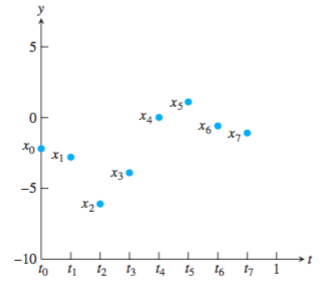
\includegraphics[width=6cm]{figs/10-2-1_DFT_Interp-1} 
%\caption{$f(x) = x^3 + x -1$的图像} 
\end{figure}
\end{frame}


\begin{frame}
\frametitle{三角插值}
令$y = F_n x$是向量$x$的傅立叶变换。由于$x$又是$y$的傅立叶逆变换,因此我们可以将$x$的分量$x_j$写为
\begin{align}
x_j = \frac{1}{\sqrt{n}} \sum_{k = 0}^{n-1} y_k (\omega^{-k})^j 
     = \frac{1}{\sqrt{n}} \sum_{k = 0}^{n-1} y_k e^{i 2\pi\frac{kj}{n}} 
     = \sum_{k = 0}^{n-1} y_k \frac{e^{i 2\pi k \frac{t_j - c}{d-c}}}{\sqrt{n}}.
\end{align}
通过上面的式子我们可以看到,如果我们将
\begin{equation}
 \frac{e^{i 2\pi k \frac{t - c}{d-c}}}{\sqrt{n}},
\end{equation}
作为插值基函数,那么
\begin{equation}
x = \sum_{k = 0}^{n-1} y_k \frac{e^{i 2\pi k \frac{t - c}{d-c}}}{\sqrt{n}},
\end{equation}
恰好对点$(t_j, x_j)$进行了插值,而$x$的离散傅立叶变换$y$的各分量正好是插值基函数前面的系数。
\end{frame}


\begin{frame}
\frametitle{离散傅立叶变换插值定理}
\begin{theorem}[离散傅立叶变换插值定理]
\label{thm: DFT interp 1}
给定区间$[c,d]$以及正数$n$,令$t_j = c + j\frac{d-c}{n}$,$j = 0, \ldots, n-1$,令$x = [x_0, \ldots, x_{n-1}]$是由$n$个数(实数或者复数)组成的向量。设$a + b i = F_n x$,其中$F_n$是离散傅立叶变换矩阵。那么函数
\begin{equation}
Q(t) = \frac{1}{\sqrt{n}} \sum_{k = 0}^{n-1} (a_k + i b_k) e^{i 2\pi k \frac{t - c}{d-c}}
\end{equation}
满足$Q(t_j) = x_j$,$j = 0, \ldots, n-1$。进一步的,如果$x_j$是实数,则以下实值函数
\begin{equation}
P(t) = \frac{1}{\sqrt{n}} \sum_{k=0}^{n-1} \big(a_k \cos \frac{2 \pi k (t-c)}{d-c} - b_k \sin \frac{2 \pi k (t-c)}{d-c}  \big)
\end{equation}
满足$P(t_j) = x_j$,$j = 0, \ldots, n-1$。
\end{theorem}
\end{frame}


\begin{frame}
\frametitle{离散傅立叶变换插值定理}
根据引理\ref{thm: DFT Property 1}中离散傅立叶变换的性质,我们可以进一步简化上式中系数的的计算,事实上,如果$n = 2m$是一个偶数,我们只需要计算$k = 0, \ldots, \frac{n}{2} -1$时$a_k$和$b_k$的值,即可得到满足$P(t_j) = x_j$,$j = 0, \ldots, n-1$的另外一个$P$的表达式:
\begin{theorem}[离散傅立叶变换插值定理]
\label{thm: DFT interp 2}
假设$n$是一个偶数,令$t_j = c + j\frac{d-c}{n}$,$j = 0, \ldots, n-1$,令$x = [x_0, \ldots, x_{n-1}]$是由$n$个实数组成的向量。设$a + b i = F_n x$,其中$F_n$是离散傅立叶变换矩阵。那么函数
\begin{align}
P(t) = &P_n(t) =  \frac{a_0}{\sqrt{n}} + \frac{2}{\sqrt{n}} \sum_{k=1}^{\frac{n}{2}-1} \big(a_k \cos \frac{2 \pi k (t-c)}{d-c} - b_k \sin \frac{2 \pi k (t-c)}{d-c}  \big) \nonumber \\
       &+ \frac{a_{\frac{n}{2}}}{\sqrt{n}} \cos \frac{n\pi(t-c)}{d-c},
\end{align}
满足$P_n(t_j) = x_j$.
\end{theorem}
\end{frame}


\begin{frame}
\frametitle{离散傅立叶变换插值定理}
\begin{remark}
\begin{enumerate}
\item 我们注意到,定理\ref{thm: DFT interp 1}和定理\ref{thm: DFT interp 2}中的$P(t)$是不同的函数,而并非是定理\ref{thm: DFT interp 2}中的$P(t) = P_n(t)$是定理\ref{thm: DFT interp 1}中的$P(t)$的化简。但是这两个函数都满足$P(t_j) = x_j$,$j = 0, \ldots, n-1$。这说明与多项式插值不同,三角插值并没有唯一性。
\item 因为计算方便,我们一般使用的是定理\eqref{thm: DFT interp 2}中的插值函数,并称这个插值公式为$n$次的三角插值函数。
\end{enumerate}
\end{remark}
\end{frame}


\begin{frame}
\frametitle{三角插值举例}
\begin{example}
对序列$x = [-2.2, -2.8, -6.1, -3.9, 0.0, 1.1, -0.6, -1.1]$在$[0,1]$上进行插值。(仔细观察可以发现这恰好是上一讲中周期性数据拟合中对一天气温拟合的问题)
\end{example}
首先找到$x$的离散傅立叶变换
\begin{figure}
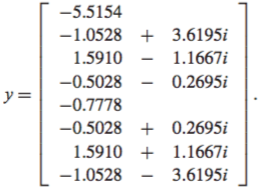
\includegraphics[width=5cm]{figs/10-2-1_DFT_Interp-2} 
%\caption{$f(x) = x^3 + x -1$的图像} 
\end{figure}
\end{frame}


\begin{frame}
\frametitle{三角插值举例}
根据三角插值公式,我们只需要前一半的傅立叶变换系数,可以得到
\begin{figure}
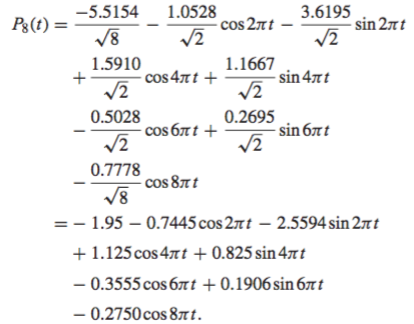
\includegraphics[width=7.5cm]{figs/10-2-1_DFT_Interp-3} 
%\caption{$f(x) = x^3 + x -1$的图像} 
\end{figure}
\end{frame}



\begin{frame}
\frametitle{三角插值举例}
插值效果如下图
\begin{figure}
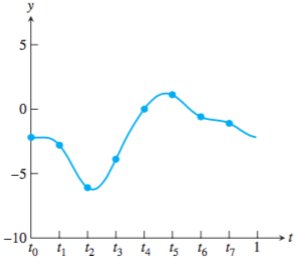
\includegraphics[width=6.5cm]{figs/10-2-1_DFT_Interp-4} 
%\caption{$f(x) = x^3 + x -1$的图像} 
\end{figure}
\end{frame}

%%%%%%%%%%%%%%%%%%%%%%%%%%%%%%%%%%%%%%%%%%



\section{正交插值和三角函数最小二乘拟合}

\subsection{正交插值}

\begin{frame}
\frametitle{正交插值和三角函数最小二乘拟合}
这一部分中,我们考虑利用某些特定基函数在插值点上的正交性进行函数插值,这实际上解释了我们上一节中利用三角函数对周期性数据进行拟合最终可以得到系数矩阵为对角阵的法方程的原因。我们还将利用这个性质推导出由三角函数进行最小二乘拟合的方便之处。

\vspace{0.2cm}

首先,我们定义正交矩阵
\begin{definition}[正交矩阵]
如果一个矩阵$U$满足
\begin{equation}
U^T U = U U^T = I,
\end{equation}
或$U^{-1} = U^T$,则这个矩阵被称为正交矩阵。正交矩阵的特点是,它的行向量或列向量之间两两正交(垂直),而每个行向量或者列向量的长度为$1$。
\end{definition}
一个简单的正交矩阵是
\begin{align*}
 \left[ \begin{array}{cc}
     \cos \phi    & \sin \phi   \\
     \sin \phi   &  -\cos \phi                   
            \end{array} \right] .
\end{align*}
\end{frame}


\begin{frame}
\frametitle{正交插值}
\begin{theorem}[正交插值定理]
\label{thm: orthogonal interp 1}
令$f_0(t), \ldots, f_{n-1}(t)$是关于实数$t$的实值函数,$t_0, \ldots, t_{n-1}$是实数。假设$n \times n$的矩阵
\begin{align}
A = \left[ \begin{array}{cccc}
     f_0(t_0)    & f_0(t_1) & \cdots  & f_0(t_{n-1})  \\
     f_1(t_0)    & f_1(t_1) & \cdots  & f_1(t_{n-1})  \\
     \vdots       & \vdots   &  \quad  & \vdots  \\
     f_{n-1}(t_0)    & f_{n-1}(t_1) & \cdots  & f_{n-1}(t_{n-1})  \\                
            \end{array} \right] ,
\end{align}
是一个实的$n \times n$的正交矩阵。令$y = Ax$,那么函数
\begin{equation}
F(t) = \sum_{k = 0}^{n-1} y_k f_k(t),
\end{equation}
对点$(t_0, x_0)$, \ldots, $(t_{n-1}, x_{n-1})$,进行了插值,即$F(t_j) = x_j$, $j = 0, \ldots, n-1$。
\end{theorem}
\end{frame}


\begin{frame}
\frametitle{正交插值}
可以看到,上面定理当中最难以满足的条件是矩阵$A$的正交性,如果随便选取函数$f(t)$和点$t_j$是很难满足$A$的正交性的。但是我们如果将函数$f(t)$选为三角函数,点$t_j$为某些等距点,则这个条件就可以满足。我们首先有如下引理:
\begin{lemma}
\label{thm: orthogonality of trigonometric functions 1}
令$n \ge 1$,$k,l$为整数,则有如下等式成立
\begin{figure}
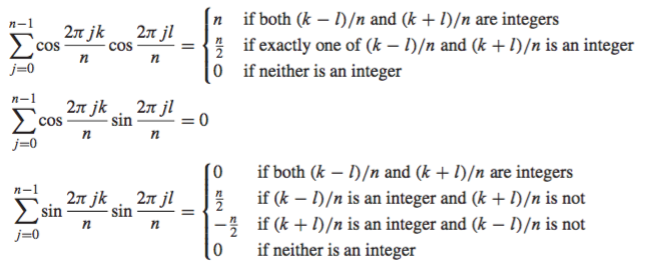
\includegraphics[width=10cm]{figs/10-3-1_Orthogonal_Interp-1} 
%\caption{$f(x) = x^3 + x -1$的图像} 
\end{figure}
\end{lemma}
\end{frame}


\begin{frame}
\frametitle{正交插值}
现在令$[c,d]$为插值区间,$n$为一个正的偶数,$t_j = c + j \frac{d-c}{n}$,$j = 0, \ldots, n-1$。令
\begin{align}
f_0(t) &= \sqrt{\frac{1}{n}} \nonumber \\
f_1(t) &= \sqrt{\frac{2}{n}} \cos \frac{2 \pi (t-c)}{d-c}, f_2(t) = \sqrt{\frac{2}{n}} \sin \frac{2 \pi (t-c)}{d-c} \nonumber \\
f_3(t) &= \sqrt{\frac{2}{n}} \cos \frac{4 \pi (t-c)}{d-c}, f_4(t) = \sqrt{\frac{2}{n}} \sin \frac{4 \pi (t-c)}{d-c} \nonumber \\
\vdots \nonumber \\
f_{n-1} (t) &= \sqrt{\frac{1}{n}} \cos \frac{n \pi (t-c)}{d-c}.
\end{align}
\end{frame}


\begin{frame}
\frametitle{正交插值}
则矩阵$A$的表达式为
\begin{align}
A =\frac{\sqrt{2}}{n} \left[ \begin{array}{cccc}
     \frac{1}{\sqrt{2}}    &  \frac{1}{\sqrt{2}}  & \cdots  & \frac{1}{\sqrt{2}}  \\
     1    & \cos \frac{2\pi}{n} & \cdots  & \cos \frac{2\pi (n-1)}{n}  \\
     0    & \sin \frac{2\pi}{n} & \cdots  & \sin \frac{2\pi (n-1)}{n}  \\     
     \vdots       & \vdots   &  \quad  & \vdots  \\
     \frac{1}{\sqrt{2}}   & \frac{1}{\sqrt{2}} \cos \pi &  \cdots  &  \frac{1}{\sqrt{2}} \cos (n-1) \pi  \\                
            \end{array} \right] .
\end{align}
可以利用引理\ref{thm: orthogonality of trigonometric functions 1}证明矩阵$A$是一个正交矩阵。
\end{frame}


\begin{frame}
\frametitle{正交插值}
有了这个结论,我们可以很容易得到,如果给定一个序列$x$,函数
\begin{align}
\label{eq: orthogonal interp trigonometric 1} 
F(t) = &\sqrt{\frac{1}{n}} y_0 \nonumber \\
       &+ y_1 \sqrt{\frac{2}{n}}  \cos \frac{2 \pi (t-c)}{d-c} + y_2 \sqrt{\frac{2}{n}}  \sin \frac{2 \pi (t-c)}{d-c} \nonumber \\
       &+ y_3 \sqrt{\frac{2}{n}} \cos \frac{4 \pi (t-c)}{d-c} +y_4  \sqrt{\frac{2}{n}} \sin \frac{4 \pi (t-c)}{d-c} \nonumber \\
\vdots \nonumber \\
       &+ y_{n-1} \sqrt{\frac{1}{n}} \cos \frac{n \pi (t-c)}{d-c},
\end{align}
是过点$(t_j = c + j \frac{d-c}{n}, x_j)$的三角插值,其中$y = Ax$。这个表达式与定理\ref{thm: DFT interp 2}中的$P_n(t)$是一模一样的。这两个公式只是导出的出发点不同,简单的总结:$P_n(t)$是通过离散傅立叶变换和离散傅立叶逆变换的性质通过对系数的简化得到的,而$F(t)$是通过特殊函数和特殊插值点的选取根据正交插值定理得到的。
\end{frame}


\begin{frame}
\frametitle{正交插值举例}
\begin{example}
\label{example: orthogonal trigonometric interp 1}
利用\eqref{eq: orthogonal interp trigonometric 1} 中的插值公式对序列$x = [-2.2, -2.8, -6.1, -3.9, 0.0, 1.1, -0.6, -1.1]$在$[0,1]$上进行插值。
\end{example}
首先求系数$y = Ax$,即
\begin{figure}
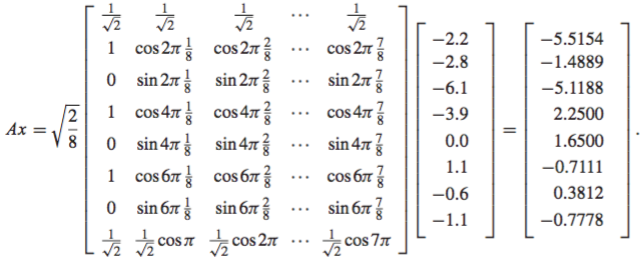
\includegraphics[width=10cm]{figs/10-3-1_Orthogonal_Interp-2} 
%\caption{$f(x) = x^3 + x -1$的图像} 
\end{figure}
\end{frame}


\begin{frame}
\frametitle{正交插值举例}
利用\eqref{eq: orthogonal interp trigonometric 1} 中的插值公式得到
\begin{figure}
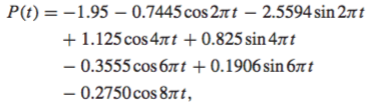
\includegraphics[width=6.5cm]{figs/10-3-1_Orthogonal_Interp-3} 
%\caption{$f(x) = x^3 + x -1$的图像} 
\end{figure}
这个结果于之前的例子也是一样的。
\end{frame}


\subsection{三角函数最小二乘拟合}

\begin{frame}
\frametitle{最小二乘拟合回顾}
回忆插值与拟合的区别,如果我们面对的是数量非常庞大的数据点,那么与其进行插值,不如利用简单函数对数据进行拟合,找到数据的趋势。回忆上一讲当中数据的最小二乘拟合问题,尤其是利用多项式函数对数据进行最小二乘拟合的问题,事实上我们相当于做了这样一件事情:利用给定的基函数$f_0(t), \ldots, f_{m-1}(t)$,找到系数$c_k$,在给定的数据点$(t_j, x_j)$, $j = 0, \ldots, n-1$上,使得函数
\begin{equation}
F_m(t) = \sum_{k = 0}^{m-1}c_k f_k(t)
\end{equation}
与$x_j$之差的二乘最小,即最小化$\sum_{j = 0}^{n-1} e_j^2 = \big(x_j - F_m(t_j)\big)$,其中$m < n$(如果$m = n$就是正好插值问题了)。
\end{frame}



\begin{frame}
\frametitle{最小二乘拟合回顾}
上面这个问题的解决方法是首先代入数据$(t_j, x_j)$,建立超定方程组
\begin{align}
\sum_{k = 0}^{m-1} c_k f_k(t_j) &= x_j, \nonumber \\
A_m^T c &= x.
\end{align}
其中
\begin{align}
A_m^T = \left[ \begin{array}{cccc}
     f_0(t_0)    & f_1(t_0) & \cdots  &   f_{m-1}(t_0) \\
      f_0(t_1)   & f_1(t_1) & \cdots  &   f_{m-1}(t_1)  \\
     \vdots       & \vdots   &  \quad  & \vdots  \\
    f_0(t_{n-1})    & f_1(t_{n-1})& \cdots  & f_{m-1}(t_{n-1})  \\                
            \end{array} \right] .
\end{align}
\end{frame}


\begin{frame}
\frametitle{最小二乘拟合回顾}
之后我们解
\begin{align}
A_m A_m^T c = A_m x
\end{align}
得到$c$,其中
\begin{align}
A_m = \left[ \begin{array}{cccc}
     f_0(t_0)    & f_0(t_1) & \cdots  & f_0(t_{n-1})  \\
     f_1(t_0)    & f_1(t_1) & \cdots  & f_1(t_{n-1})  \\
     \vdots       & \vdots   &  \quad  & \vdots  \\
     f_{m-1}(t_0)    & f_{m-1}(t_1) & \cdots  & f_{m-1}(t_{n-1})  \\                
            \end{array} \right] .
\end{align}
如果仔细观察,可以发现,$A_m$恰好是定理\ref{thm: orthogonal interp 1}中的$A$的前$m$行。如果我们选择$f_0, \ldots, f_{n-1}$和$t_0, \ldots, t_{n-1}$使得$A$矩阵是正交矩阵,那么根据正交矩阵的性质,它的行向量之间也是两两正交的,从而$A_m A_m^T = I$,最终可以得到
\begin{equation}
c = A_m x.
\end{equation}
\end{frame}


\begin{frame}
\frametitle{正交函数最小二乘拟合定理}
我们有以下定理
\begin{theorem}[正交函数插值和最小二乘拟合定理]
\label{thm: orthogonal interp and least square fit 1}
令$m<n$是一个整数并给定数据点$(t_0, x_0), \ldots, (t_{n-1}, x_{n-1})$。令$y = Ax$,其中$A$在定理\ref{thm: orthogonal interp 1}中给出,且$A$是正交矩阵。那么由基函数$f_0(t), \ldots, f_{n-1}(t)$确定的插值函数的表达式是
\begin{equation}
F_n(t) = \sum_{k=0}^{n-1} y_k f_k(t).
\end{equation}
如果我们只利用前$m$个基函数$f_0(t), \ldots, f_{n-1}(t)$对数据点进行拟合,则得到最小二乘意义下的最佳拟合函数为
\begin{equation}
F_m(t) = \sum_{k=0}^{m-1} y_k f_k(t).
\end{equation}
\end{theorem}
\end{frame}


\begin{frame}
\frametitle{正交函数最小二乘拟合举例}
事实上,定理\ref{thm: orthogonal interp and least square fit 1}中的结论还有一个重要的好处,就是我们如果我们恰当的选择了基函数与数据点的$t$值,那么每次我们增加一个基函数,之前的基函数前面的系数是不变的。例如对周期性数据的进行拟合问题中(例\ref{example: orthogonal trigonometric interp 1}),我们可以观察到
\begin{figure}
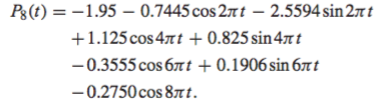
\includegraphics[width=6.5cm]{figs/10-3-2_Orthogonal_Interp-1} 
%\caption{$f(x) = x^3 + x -1$的图像} 
\end{figure}
而
\begin{figure}
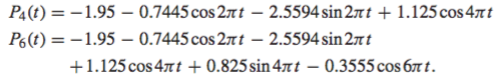
\includegraphics[width=8cm]{figs/10-3-2_Orthogonal_Interp-2} 
%\caption{$f(x) = x^3 + x -1$的图像} 
\end{figure}
\end{frame}


\begin{frame}
\frametitle{三角函数最小二乘拟合}
应该如何选取函数$f_k(t)$与点$t_j$呢?其实我们早已经给出了答案,这就是对于区间$[c,d]$上的数据进行拟合,我们取$t_j = c + j \frac{d-c}{n}$,$j = 0, \ldots, n-1$,$x_j$为这些点上的测量值,而
\begin{align}
f_0(t) &= \sqrt{\frac{1}{n}} \nonumber \\
f_1(t) &= \sqrt{\frac{2}{n}} \cos \frac{2 \pi (t-c)}{d-c}, f_2(t) = \sqrt{\frac{2}{n}} \sin \frac{2 \pi (t-c)}{d-c} \nonumber \\
f_3(t) &= \sqrt{\frac{2}{n}} \cos \frac{4 \pi (t-c)}{d-c}, f_4(t) = \sqrt{\frac{2}{n}} \sin \frac{4 \pi (t-c)}{d-c} \nonumber \\
\vdots \nonumber \\
f_{n-1} (t) &= \sqrt{\frac{1}{n}} \cos \frac{n \pi (t-c)}{d-c}.
\end{align}
\end{frame}


\begin{frame}
\frametitle{三角函数最小二乘拟合}
由定理\ref{thm: DFT interp 2}中的$P_n(t)$与\eqref{eq: orthogonal interp trigonometric 1} 中$F(t)$的等价性,我们很容易得到以下推论
\begin{theorem}
考虑$[c,d]$区间,假设$m<n$且$m,n$都是偶数,令$t_j = c + j\frac{d-c}{n}$,$j = 0, \ldots, n-1$,令$x = [x_0, \ldots, x_{n-1}]$是由$n$个实数组成的向量。设$a + b i = F_n x$,其中$F_n$是离散傅立叶变换矩阵。那么函数
\begin{align}
P_m(t) = &  \frac{a_0}{\sqrt{n}} + \frac{2}{\sqrt{n}} \sum_{k=1}^{\frac{m}{2}-1} \big(a_k \cos \frac{2 \pi k (t-c)}{d-c} - b_k \sin \frac{2 \pi k (t-c)}{d-c}  \big) \nonumber \\
       &+ \frac{a_{\frac{m}{2}}}{\sqrt{n}} \cos \frac{m\pi(t-c)}{d-c},
\end{align}
是对数据点$(t_j, x_j)$, $j = 0, \ldots, n-1$的$m$阶的最佳三角函数拟合,或者叫作最佳三角逼近。
\end{theorem}
\end{frame}


\begin{frame}
\frametitle{三角函数最小二乘拟合}
我们引入上面的推论的原因是,如果$n = 2^L$,那么系数$a_k, b_k$通过离散傅立叶变换是非常容易计算的(计算复杂度是$O(n\log n)$。因此,如果我们需要对大规模的数据进行最佳三角逼近,逼近函数的基函数又选择的比较多(例如$m^2 >n$),那么我们往往选择$n = 2^L$个等距数据点,利用离散傅立叶变换得到系数,然后把三角逼近直接通过上面推论中的公式写出来,而不再将$A_m$矩阵写出来,再通过$A_mx$求得系数,因为这样做的计算复杂度为$O(m^2)$,往往比$O(n\log n)$还要大。
\end{frame}




%%%%%%%%%%%%%%%%%%%%%%%%%%%%%%%%%%%%%%%%%%

\begin{frame}
\frametitle{课后阅读及作业}
[NA] 第10章 10.1.1,10.1.2,10.2.1,10.3.1,10.3.2\\
作业:[NA] 10.1:1,3,6;10.2: 1,3;10.3: 1,2,4。


\end{frame}

\end{document}

